\section{Server}\label{app:state-at-handoff:server}

The server is set up using Docker, and the content is divided into containers whenever possible. 
Last year they started to make the containers run in clusters. 
To do this they used Kubernetes. In the stat of the semester, only the Gitlab workers run as pots inside Kubernetes.

The Kubeneters is setup with one master node and three other nodes. Besides that, there are three non-clustered servers. \autoref{fig:app:state-at-handoff:server} shows the complete overview of the servers and which services they run.

The server hosting it self is handled by the Aalborg University IT Service Department, where every server is a virtualization using vSphere.

\begin{figure}[h]
    \centering
    \caption{Diagram of the server setup at the time of handoff}
    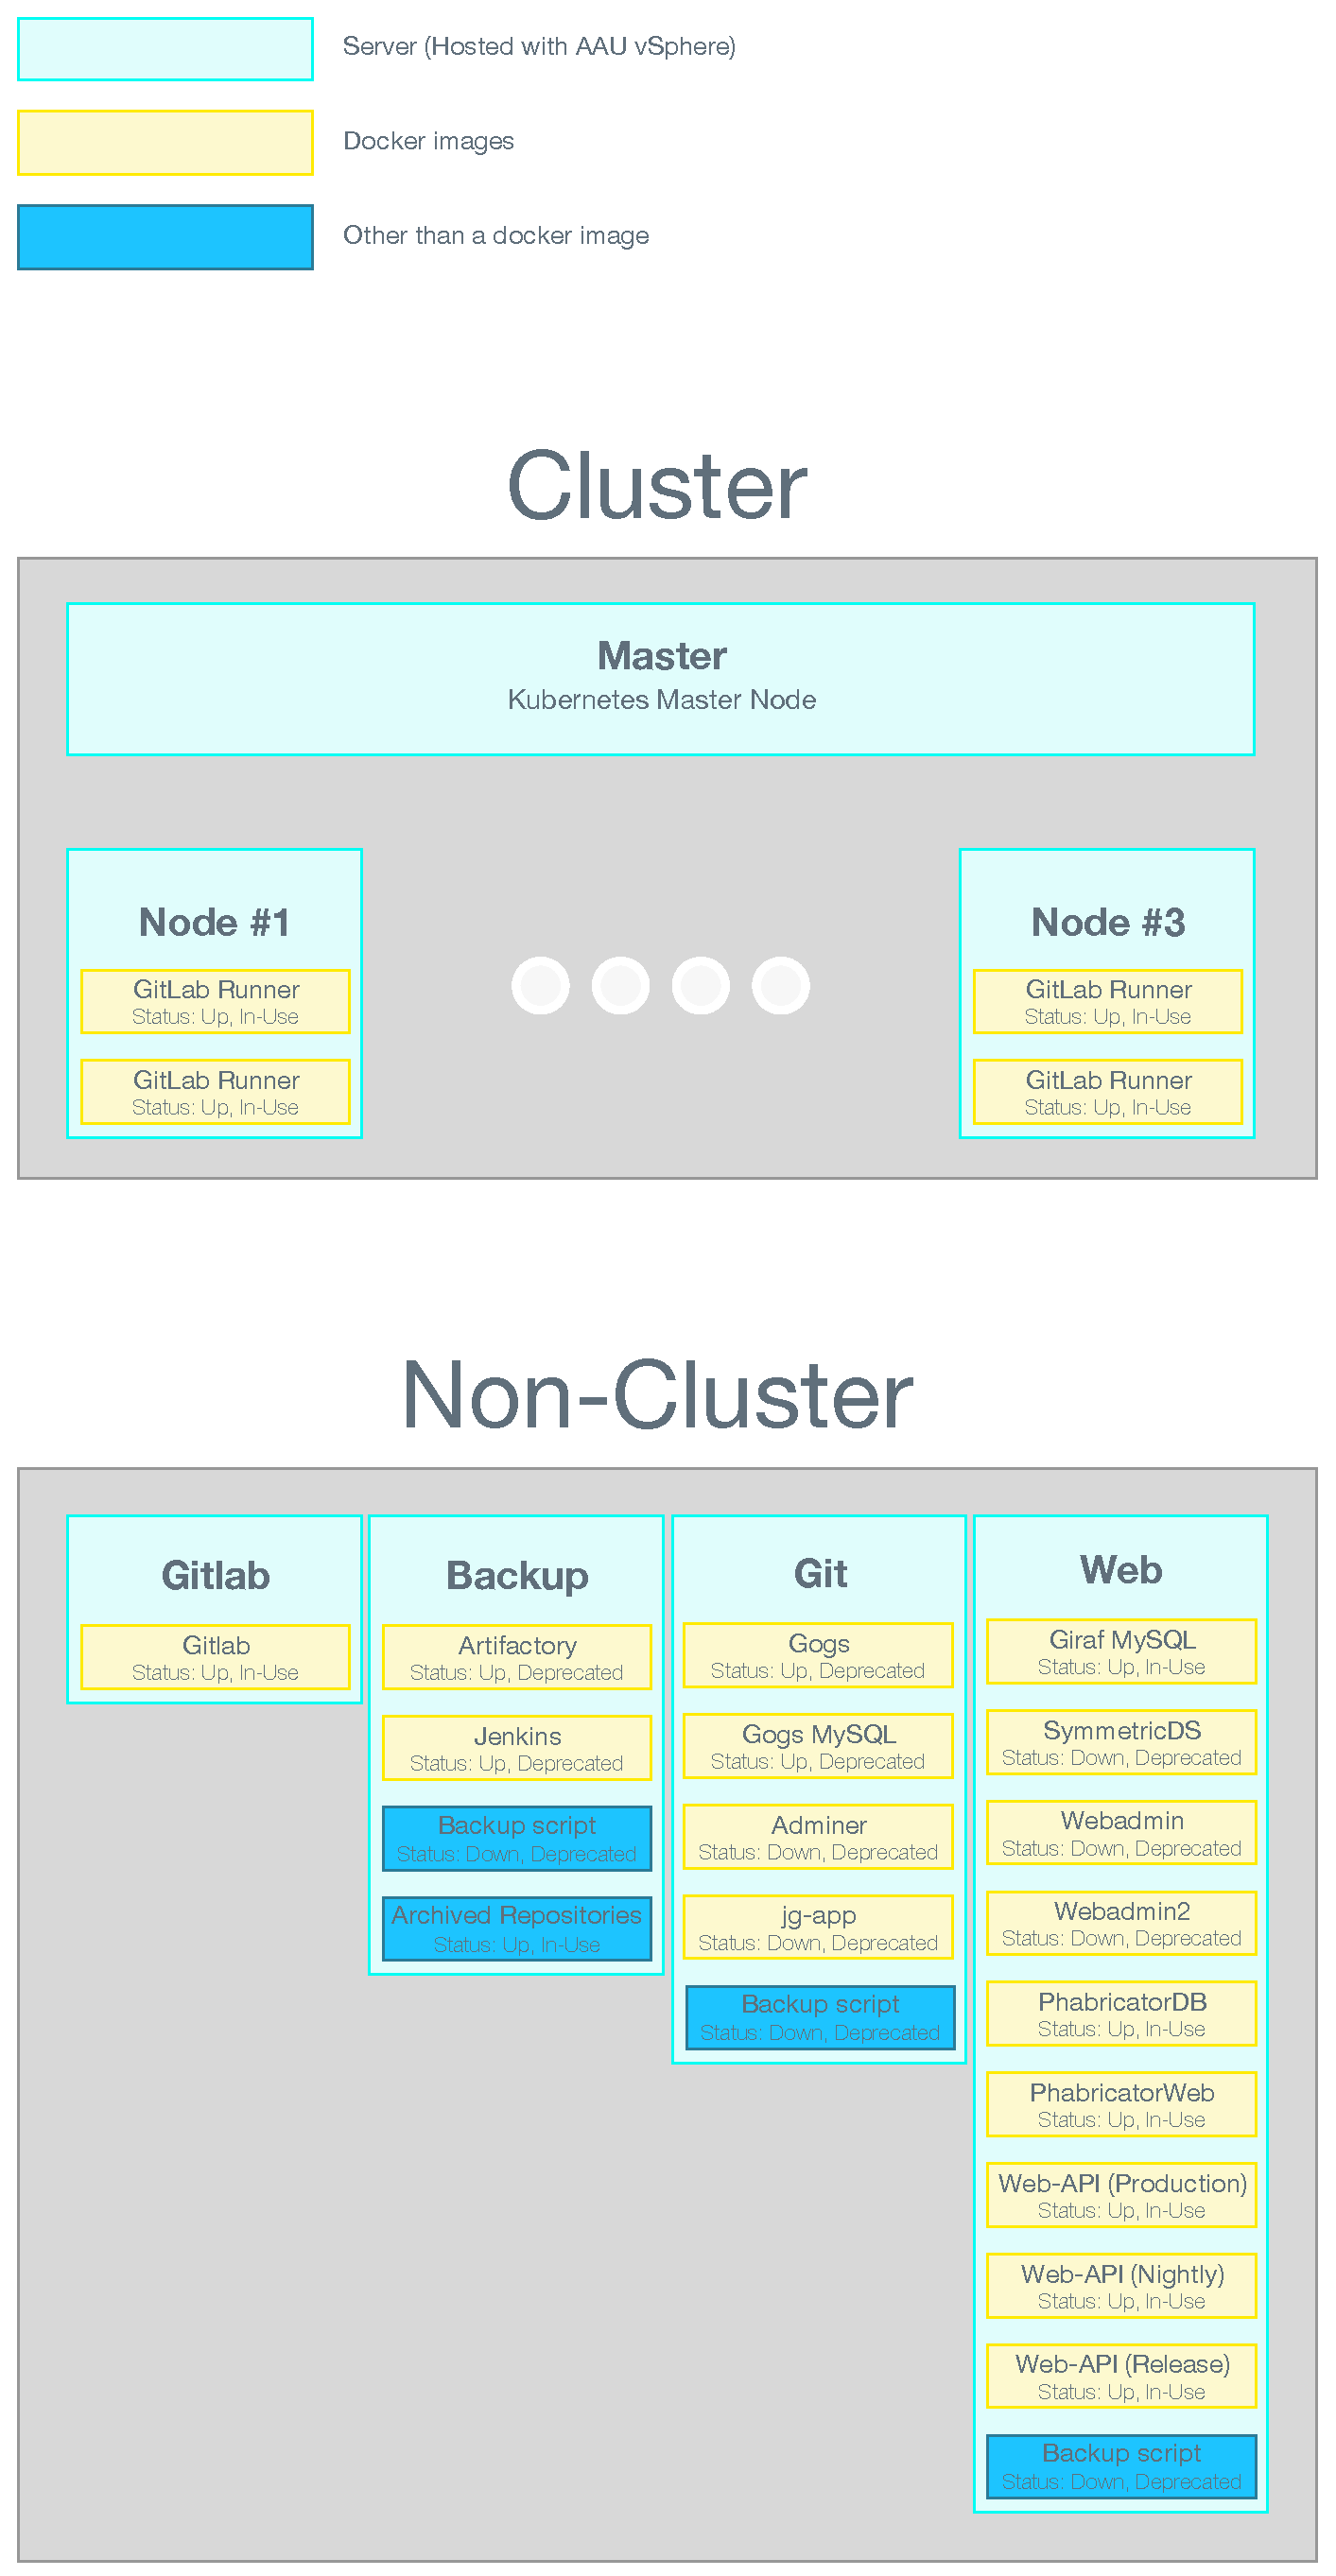
\includegraphics[height=1\textheight]{figures/Server-Overview.pdf}
    \label{fig:app:state-at-handoff:server}
\end{figure}
